%% If you have any problems using this template, please contact the author: %%
%% Chris Carmona: carmona@stats.ox.ac.uk ; chriscarmona.me %%

\documentclass{beamer}

\usepackage[UKenglish]{babel}
\usepackage[utf8]{inputenc} % so we can input characters with accents (e.g. ő)
\usepackage[export]{adjustbox}

%\usepackage{Presentation/Presentation_layout}
\usepackage{tikz}
\usetikzlibrary{calc,arrows,fadings, automata, positioning}
\tikzfading[name=fade inside,inner color=red,outer color=blue]
\usepackage{graphicx} % ease graphics management

\usefonttheme[onlymath]{serif}

%\usefonttheme{serif} % change font to allow \textbf{}
\usepackage{amsmath,amsthm,amssymb} % for math equations
\usepackage[square,sort,comma,numbers]{natbib} % richer citation
\usepackage{breakcites} % avoid overfull hbox for long cites
\definecolor{kthBlue}{RGB}{25, 84, 166}          % Oxford Blue
\definecolor{bggrey}{RGB}{240, 240, 240}          % Oxford Blue

\usepackage{bm}

\usecolortheme{beaver}
\setbeamercolor{frametitle}{fg=white,bg=kthBlue}
\setbeamercolor{title}{fg=white,bg=kthBlue}
\setbeamercolor{section in toc}{fg=kthBlue}
\setbeamercolor{background canvas}{bg=bggrey}


\DeclareMathOperator{\newdiff}{d} % use \dif instead
\newcommand{\dif}{\newdiff\!}
\newcommand{\fdif}[2]{\dfrac{\dif #1}{\dif #2}}
\newcommand{\ffdif}[2]{\dfrac{\dif^2 #1}{\dif #2^2}}
\newcommand{\fndif}[3]{\dfrac{\dif^{#3} #1}{\dif #2^{#3}}}

\newcommand{\fpart}[2]{\dfrac{\partial #1}{\partial #2}}
\newcommand{\ffpart}[2]{\dfrac{\partial^2 #1}{\partial #2^2}}
\newcommand{\fnpart}[3]{\dfrac{\partial^{#3} #1}{\partial #2^{#3}}}


%% Information (author, title, etc.) %%


\title[Short Title]{% short title for footer
    \color{white} Final project
    \vspace{0.5cm}
}

\author{Miguel De Le Court}

\institute{
        \textit{Methods in High performance computing}\\
        \textit{DD2356}
        \vspace{0.5cm}
}
\date[Venue and Date]{% short date for footer
   Stockholm, June 2021 
}

%% Content of slides %%
%%%%%%%%%%%%%%%%%%%%
\begin{document}
%%%%%%%%%%%%%%%%%%%%

% Title slide %
{
    \setbeamertemplate{footline}{}
    \setbeamertemplate{headline}{}
    \setbeamercolor{background canvas}{bg = kthBlue}
    \setbeamercolor{normal text}{fg=white}
    \usebeamercolor[fg]{normal text}
    \maketitle
}

%----------------------------%
% Contents slide
%\setbeamertemplate{background canvas}{\begin{tikzpicture} \node[opacity=.1]{\includegraphics[width=\paperwidth]{Figures/Presentation/KTH_camp.png}};\end{tikzpicture}}
% only for the image:
% Conclusions
\begin{frame}{Outline}
\tableofcontents

\vfill
\begin{center}
    \footnotesize The last version of these slides and the code presented here are available at \url{https://github.com/MiguelDLC/DD2356-Project}    
\end{center}

\end{frame}
%----------------------------%

%now include the slides
\setbeamercovered{transparent}
%----------------------------%



% Introduction
%----------------------------%
\section{Structure of the code}
\begin{frame}{Structure of the code}
    \begin{figure}
        \centering
        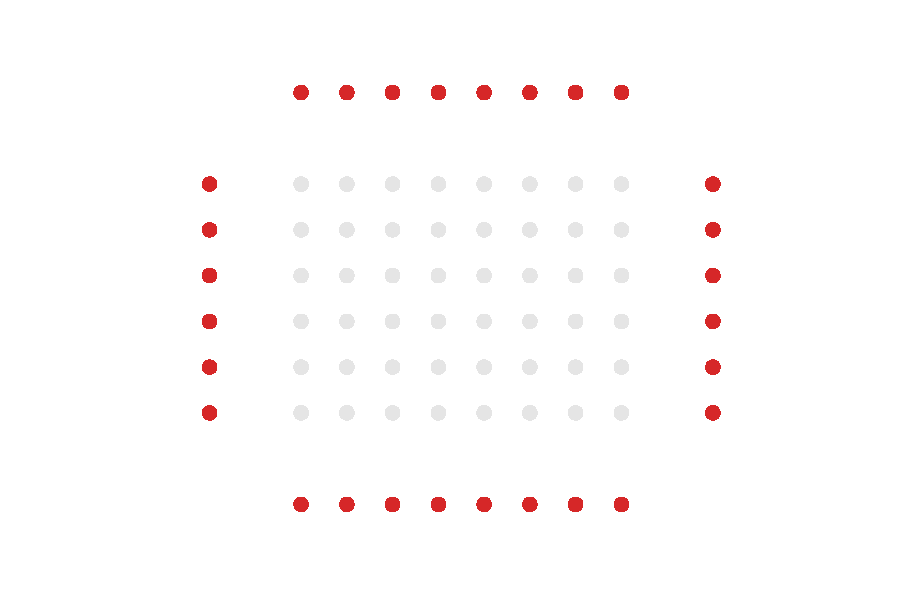
\includegraphics[width=0.8\linewidth]{Figures/step0.pdf}
    \end{figure}
\end{frame}

%----------------------------%

\begin{frame}{Structure of the code}
    \begin{figure}
        \centering
        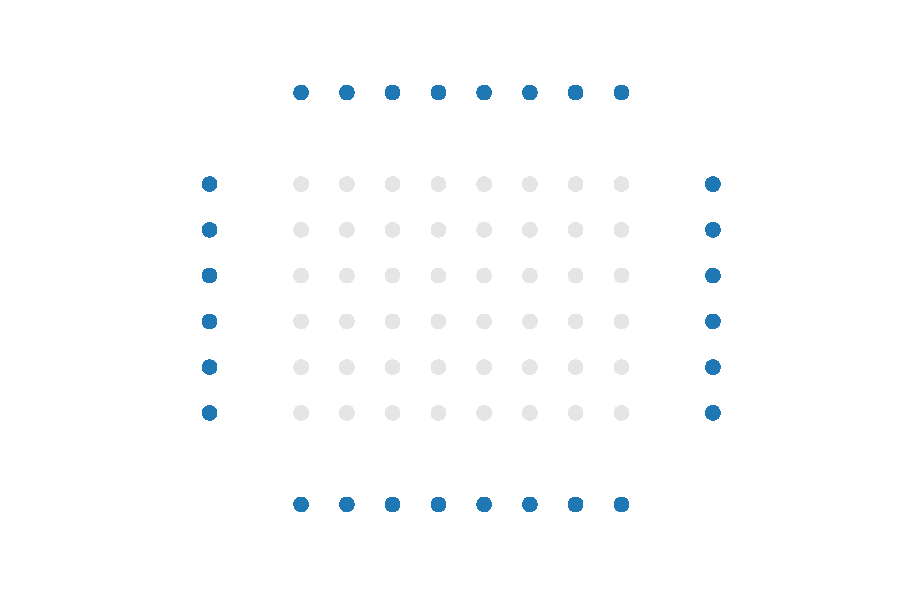
\includegraphics[width=0.8\linewidth]{Figures/step1.pdf}
    \end{figure}
\end{frame}

%----------------------------%

\begin{frame}{Structure of the code}
    \begin{figure}
        \centering
        
\includegraphics[width=0.8\linewidth]{Figures/step2.pdf}
    \end{figure}
\end{frame}

%----------------------------%

\begin{frame}{Structure of the code}
    \begin{figure}
        \centering
        
\includegraphics[width=0.8\linewidth]{Figures/step3.pdf}
    \end{figure}
\end{frame}

%----------------------------%


\begin{frame}{Structure of the code}
    \begin{figure}
        \centering
        
\includegraphics[width=0.8\linewidth]{Figures/step4.pdf}
    \end{figure}
\end{frame}

%----------------------------%


\section{Validation}
\subsection{Reference implementation}
\begin{frame}{Validation}
    Result computed with the MPI solver
    \begin{figure}
        \centering
        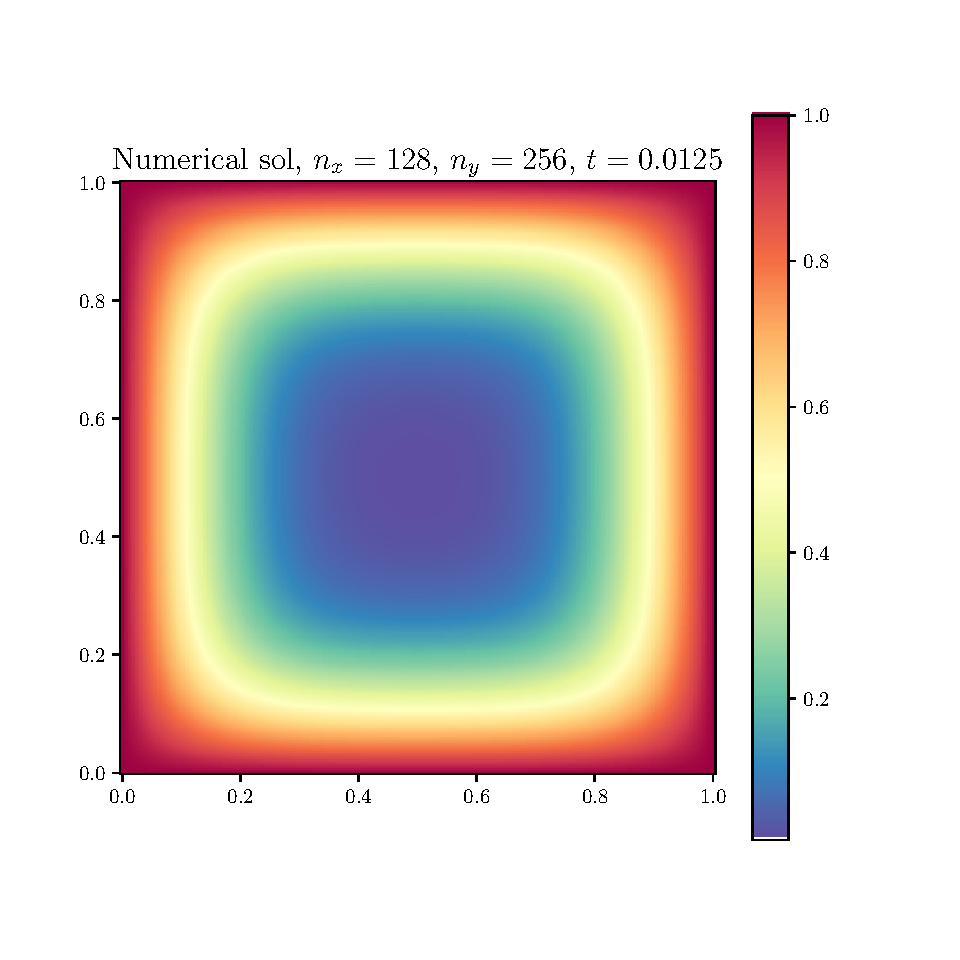
\includegraphics[height=8cm]{Figures/sol.pdf}
    \end{figure}
\end{frame}

%----------------------------%

\begin{frame}{Validation}
    \framesubtitle{Comparison with a reference implementation}
    First validation test : check against a reference implementation
    \begin{figure}
        \centering
        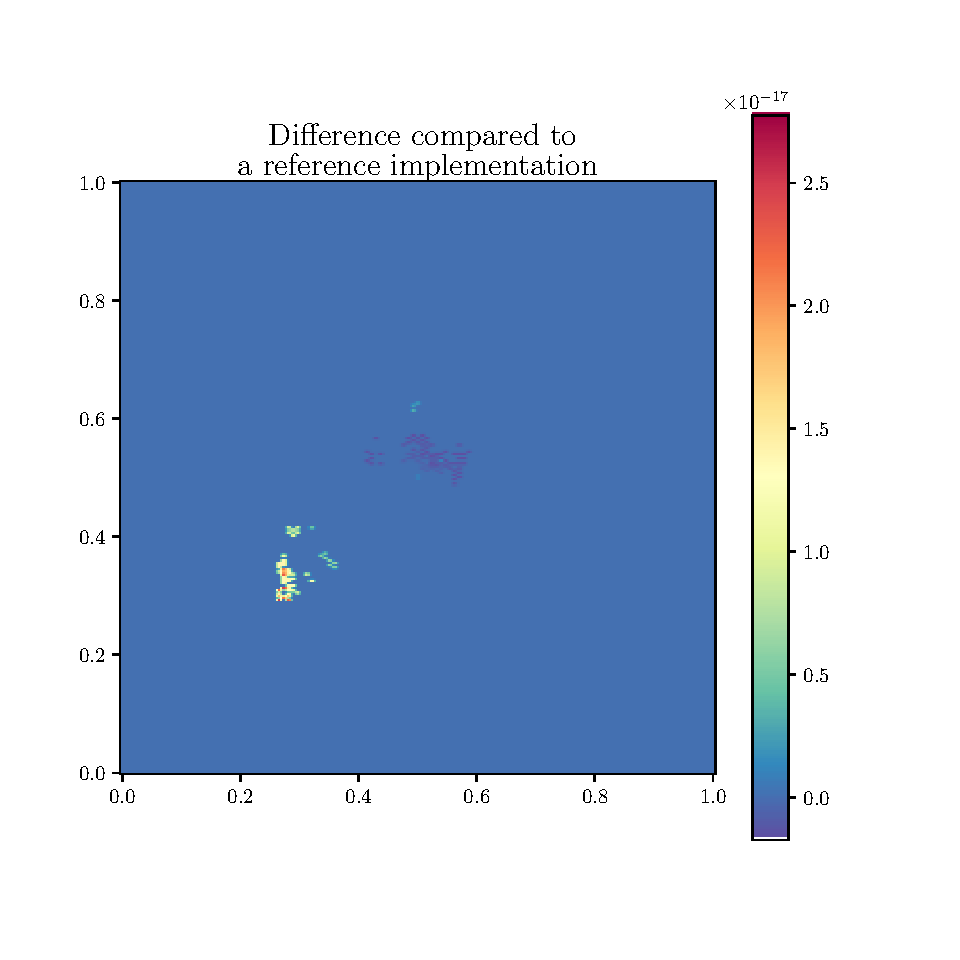
\includegraphics[height=8cm]{Figures/solcomp.pdf}
    \end{figure}
\end{frame}

%----------------------------%

\subsection{Comparison with the analytical solution}
\begin{frame}{Validation}
    \framesubtitle{Comparison with an analytical solution}
    Second validation test : check against a reference implementation and ensure that the erro decreases as expected

    \begin{figure}
        \centering
        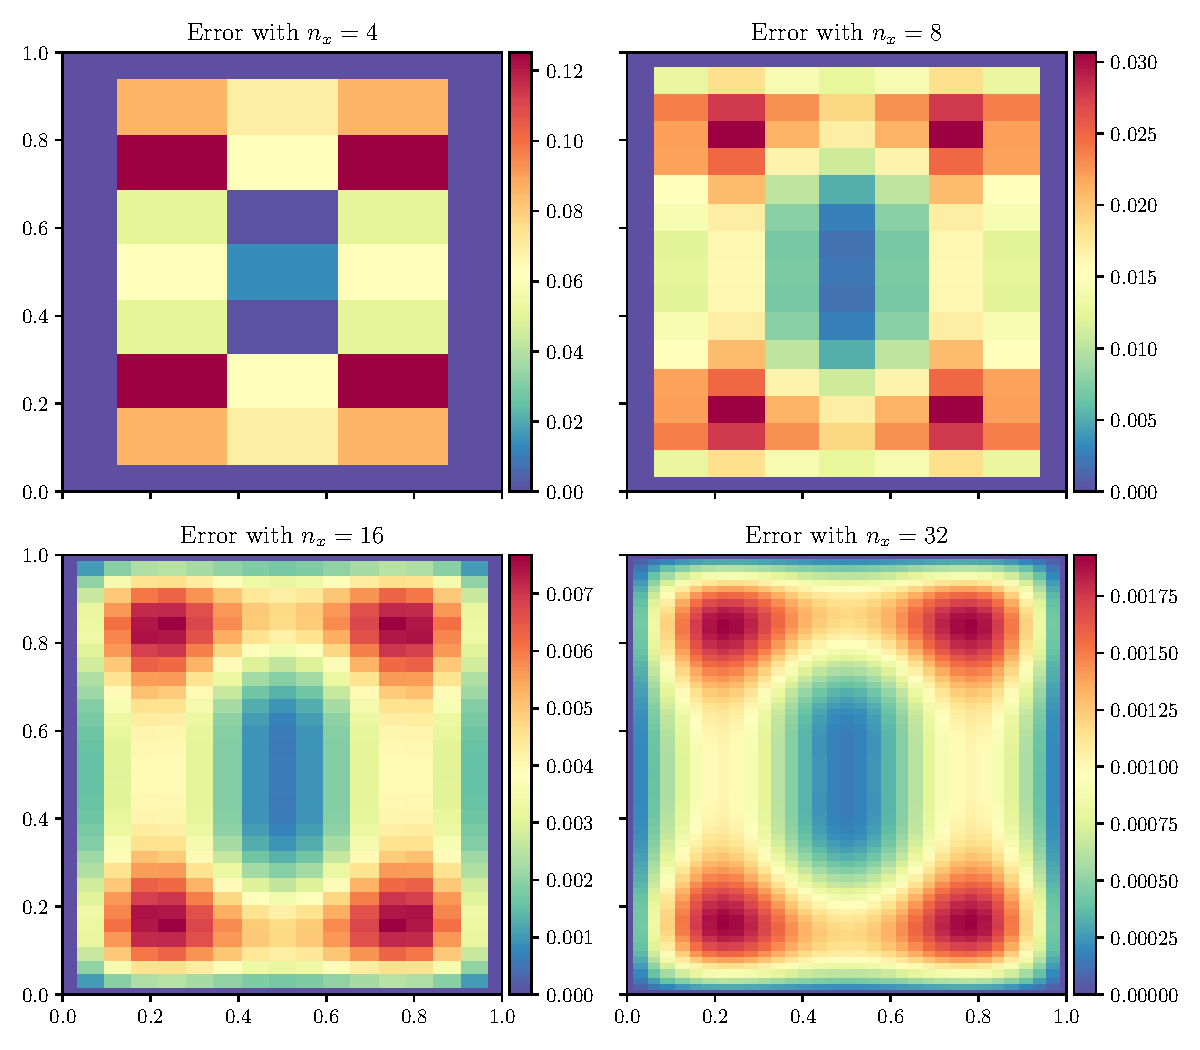
\includegraphics[height=7cm]{Figures/plotconverge.pdf}
    \end{figure}
\end{frame}

%----------------------------%

\begin{frame}{Validation}
    \framesubtitle{Comparison with an analytical solution}
    Second validation test : check against a reference implementation and ensure that the erro decreases as expected

    \begin{figure}
        \centering
        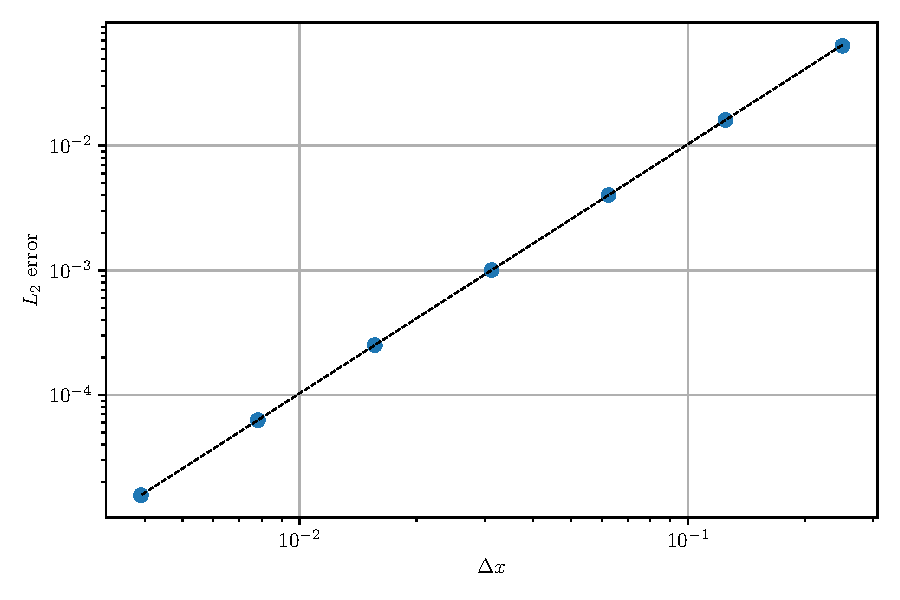
\includegraphics[width=0.8\linewidth]{Figures/Convergence.pdf}
    \end{figure}
\end{frame}

%----------------------------%

\section{Idle propagation}
\begin{frame}{Idle propagation}
    \framesubtitle{Comparison with an analytical solution}
    \begin{figure}
        \centering
        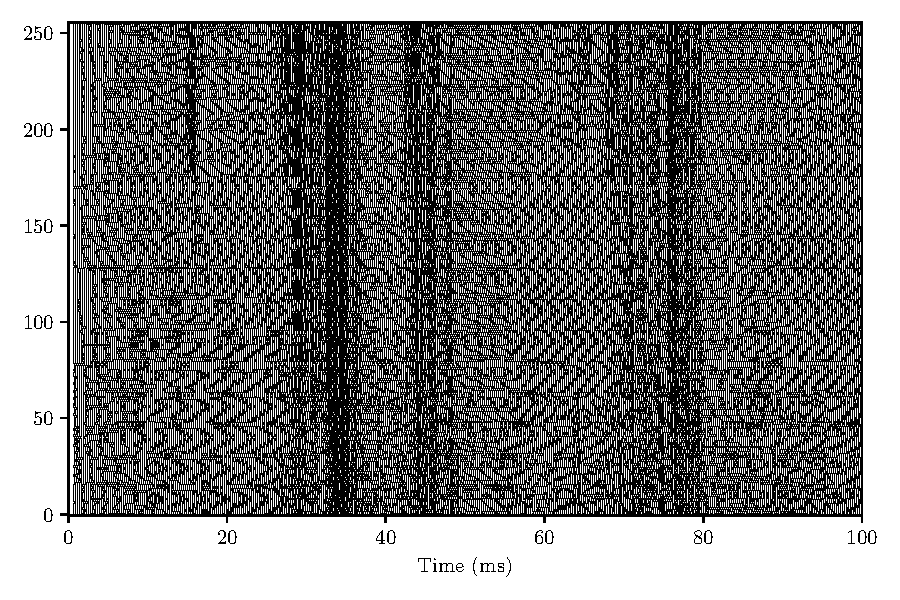
\includegraphics[width=0.8\linewidth]{Figures/idle_propagation.pdf}
    \end{figure}
\end{frame}

%----------------------------%

\begin{frame}{Idle propagation}
    \framesubtitle{Comparison with an analytical solution}
    \begin{figure}
        \centering
        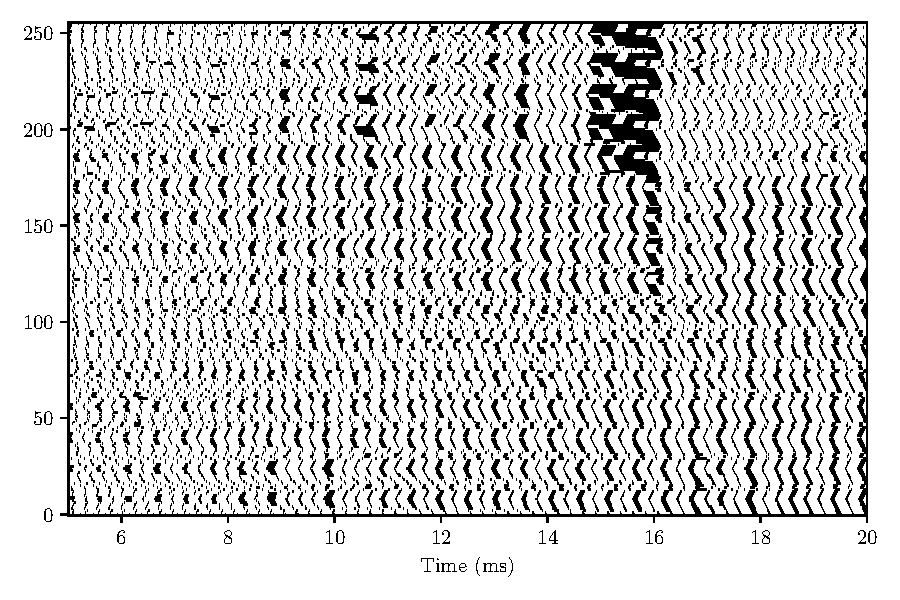
\includegraphics[width=0.8\linewidth]{Figures/idle_propagation_small.pdf}
    \end{figure}
\end{frame}

%%%%%%%%%%%%%%%%%%%%
\end{document}
%%%%%%%%%%%%%%%%%%%%
